\chapter{Equilibrios redox y ecuación de Nernst}\label{ch:b1:nernst}

Se introduce una lámina de cinc en una disolución de sulfato de cinc y
una lámina de cobre en una disolución de sulfato de cobre(II), se unen
las dos disoluciones con un tubo de disolución salina y los dos metales
con un hilo que pasa por un diodo emisor de luz: el diodo se enciende. La
reacción del cinc con los iones cobre, que en un solo vaso solo calienta
la disolución, impulsa ahora electrones por un hilo. Una batería es este
montaje, empaquetado; un pHmetro y un electrodo de cloruro son sus
parientes de medida. Este capítulo hace cuantitativo el intercambio de
electrones: los \omterm{def:b1:nernst:oxidation-number}{números de oxidación} para contar los electrones, los
\omterm{def:b1:nernst:electrode-potential}{potenciales de electrodo} para ordenar los pares y la \omterm{thm:b1:nernst:nernst}{ecuación de Nernst}
para seguirlos en función de la concentración.

\begin{recall}
El volumen escolar (años 11 y 12) definió los \omterm{def:b1:nernst:couple}{oxidantes} y los \omterm{def:b1:nernst:couple}{reductores},
escribió \omterm{def:b1:nernst:couple}{semiecuaciones}, construyó pilas con dos metales y dos
disoluciones e interpretó la pila cinc--cobre como una batería. El
\omterm{def:b1:extent-q-and-k:quotient}{cociente de reacción} y la constante de equilibrio son los del
\cref{ch:b1:extent-q-and-k}; las \omterm{def:b1:extent-q-and-k:activity}{actividades} son $c/c^\circ$ para los
solutos y $p/p^\circ$ para los gases, y 1 para los sólidos y líquidos
puros.
\end{recall}

\section{Números de oxidación y pares}

\begin{definition}[Oxidante, reductor, par redox, semiecuación]\label{def:b1:nernst:couple}
Un \emph{oxidante}\index{oxidante} es una especie capaz de ganar
electrones, y un \emph{reductor}\index{reductor}, una especie capaz de
cederlos. Un oxidante Ox y el reductor Red en el que se convierte forman
un \emph{par redox}\index{par redox} Ox/Red, descrito por su
\emph{semiecuación}\index{semiecuacion@semiecuación}
$\alpha\,\mathrm{Ox} + n\,\mathrm{e^-} \rightleftharpoons
\beta\,\mathrm{Red}$, ajustada en átomos con \ce{H2O} y \ce{H+} cuando
hace falta y en cargas con los electrones.
\end{definition}

Una reacción redox es el intercambio de electrones entre dos pares: el
\omterm{def:b1:nernst:couple}{oxidante} de uno se reduce mientras el \omterm{def:b1:nernst:couple}{reductor} del otro se oxida, y los
electrones se cancelan. Para contarlos en una especie complicada, se
asigna a cada átomo un \omterm{def:b1:nernst:oxidation-number}{número de oxidación}.

\begin{definition}[Número de oxidación]\label{def:b1:nernst:oxidation-number}
El \emph{número de oxidación}\index{numero de oxidacion@número de oxidación} de un átomo en una
especie es la carga que llevaría si todos los enlaces se rompieran
cediendo los dos electrones enlazantes al átomo más electronegativo
(repartidos por igual entre dos átomos idénticos). Se escribe en números
romanos: hierro(III), \ce{Mn^{+VII}} en el ion permanganato.
\end{definition}

\begin{proposition}[Reglas de los números de oxidación]\label{prop:b1:nernst:on-rules}
\begin{enumerate}
  \item Un átomo en un elemento tiene \omterm{def:b1:nernst:oxidation-number}{número de oxidación} 0; un ion
        monoatómico tiene su carga.
  \item Los \omterm{def:b1:nernst:oxidation-number}{números de oxidación} de los átomos de una especie suman su
        carga.
  \item El hidrógeno es $+$I (salvo en los hidruros metálicos, $-$I); el
        oxígeno es $-$II (salvo en los peróxidos, $-$I, y unido al flúor);
        el flúor es $-$I.
  \item En una \omterm{def:b1:nernst:couple}{semiecuación}, el número de electrones es igual a la
        variación del \omterm{def:b1:nernst:oxidation-number}{número de oxidación} del elemento que cambia,
        multiplicada por el número de sus átomos.
\end{enumerate}
\end{proposition}

\begin{proof}
1 y 2: romper todos los enlaces conserva la carga, y entre átomos
idénticos no se transfiere nada. 3: el hidrógeno es menos
electronegativo que todos los no metales con los que se enlaza
(\cref{ch:b1:periodicity}) y más que los metales alcalinos; el oxígeno es
más electronegativo que todos los elementos salvo el flúor, y en
\ce{O-O} el par compartido se reparte. 4: H y O conservan sus números, de
modo que los únicos átomos cuya carga ficticia cambia son los del
elemento considerado, y los electrones aparecen en la \omterm{def:b1:nernst:couple}{semiecuación}
exactamente para compensar ese cambio de carga.
\end{proof}

\begin{method}[Números de oxidación de una especie]\label{met:b1:nernst:oxidation-numbers}
Se asignan a H, O, F y a los iones sus números habituales; el número del
átomo restante se deduce de la regla 2. En \ce{MnO4-}: $x + 4(-2) = -1$,
$x = +7$. En \ce{Cr2O7^2-}: $2x - 14 = -2$, $x = +6$. En \ce{S4O6^2-}, la
media es $+2.5$; la \omterm{def:b1:lewis-resonance-vsepr:lewis}{estructura de Lewis} muestra dos tipos de azufre.
\end{method}

\begin{method}[Ajustar una semiecuación]\label{met:b1:nernst:balance-by-on}
\begin{enumerate}
  \item Se ajusta el elemento que cambia de \omterm{def:b1:nernst:oxidation-number}{número de oxidación}.
  \item Se añaden los electrones: la variación del \omterm{def:b1:nernst:oxidation-number}{número de oxidación}
        multiplicada por el número de átomos.
  \item Se ajusta la carga con \ce{H+} (disolución ácida) o con \ce{OH-}
        (disolución básica).
  \item Se ajustan el hidrógeno y el oxígeno con \ce{H2O}; el oxígeno se
        comprueba al final.
\end{enumerate}
Para el ion permanganato en medio ácido: el Mn pasa de $+$VII a $+$II,
luego 5 electrones; la carga a la izquierda es $-1 - 5 = -6$ y a la
derecha $+2$, luego $8\,\ce{H+}$; después, $4\,\ce{H2O}$:
\ce{MnO4- + 8H+ + 5e- -> Mn^2+ + 4H2O}.
\end{method}

\section{Pilas electroquímicas}

\begin{definition}[Pila electroquímica]\label{def:b1:nernst:cell}
Una \emph{pila electroquímica}\index{pila electroquimica@pila electroquímica} son dos
\emph{semipilas}\index{semipila}, cada una formada por un par y un
conductor electrónico, el electrodo, unidas por un conductor iónico, a
menudo un \emph{puente salino}\index{puente salino} (un gel o un tubo de
una sal inerte concentrada, como el nitrato de potasio). El electrodo
donde tiene lugar la oxidación es el \emph{ánodo}\index{anodo@ánodo}, y
aquel donde tiene lugar la reducción, el \emph{cátodo}\index{catodo@cátodo}.
La \emph{tensión de la pila}\index{tension de la pila@tensión de la pila} es la diferencia de
potencial eléctrico entre los dos electrodos, polo positivo menos polo
negativo, medida cuando no circula corriente.
\end{definition}

\begin{omfigure}
\begin{tikzpicture}[font=\small, >={Stealth}]
  \pic at (0,0) {beaker={0.7}{omDef!14}};
  \pic at (3.6,0) {beaker={0.7}{omDef!32}};
  \pic at (-0.3,0.25) {electrode={black!35}};
  \pic at (3.9,0.25) {electrode={orange!70!brown}};
  \pic at (0.35,0.55) {saltbridge={2.9}};
  \pic (m) at (1.8,4.3) {meter={V}};
  \draw[thick] (-0.15,2.65) |- (m-a);
  \draw[thick] (4.05,2.65) |- (m-b);
  \node[anchor=east] at (-0.95,1.0) {\ce{Zn}};
  \node[anchor=west] at (4.45,1.0) {\ce{Cu}};
  \node at (0.25,-0.35) {\ce{Zn^2+}, \ce{SO4^2-}};
  \node at (3.6,-0.35) {\ce{Cu^2+}, \ce{SO4^2-}};
  \draw[->, omProp, thick] (-0.15,3.35) -- (0.8,3.35) node[above, midway] {$\mathrm{e^-}$};
  \draw[->, omProp, thick] (2.8,3.35) -- (3.75,3.35) node[above, midway] {$\mathrm{e^-}$};
  \node[anchor=east] at (-0.9,2.3) {$-$ ánodo};
  \node[anchor=west] at (4.6,2.3) {cátodo $+$};
  \node[font=\scriptsize, align=center] at (1.8,2.75) {puente salino\\ \ce{K+} $\rightarrow$ \quad $\leftarrow$ \ce{NO3-}};
  \node[font=\scriptsize] at (-0.1,-0.8) {\ce{Zn -> Zn^2+ + 2e-}};
  \node[font=\scriptsize] at (3.7,-0.8) {\ce{Cu^2+ + 2e- -> Cu}};
\end{tikzpicture}

{\small La pila cinc--cobre (pila Daniell). El cinc se oxida en el \omterm{def:b1:nernst:cell}{ánodo},
el polo negativo; los iones cobre se reducen en el \omterm{def:b1:nernst:cell}{cátodo}, el polo
positivo. Los electrones circulan por el circuito exterior del cinc al
cobre; en el \omterm{def:b1:nernst:cell}{puente salino}, los cationes se desplazan hacia el \omterm{def:b1:nernst:cell}{cátodo} y
los aniones hacia el \omterm{def:b1:nernst:cell}{ánodo}, manteniendo neutra cada disolución.}
\end{omfigure}

Una pila se escribe en una línea, con el \omterm{def:b1:nernst:cell}{ánodo} a la izquierda: \ce{Zn}
$|$ \ce{Zn^2+}
$\|$ \ce{Cu^2+} $|$ \ce{Cu}; las barras simples indican las interfases, y
la barra doble, el \omterm{def:b1:nernst:cell}{puente salino}. Con todas las concentraciones a
\qty{1}{mol/L}, su tensión es de \qty{1.10}{V}. La reacción que tiene
lugar cuando la pila suministra corriente, \ce{Zn + Cu^2+ -> Zn^2+ + Cu},
es la misma que ocurriría en un solo vaso; separar las \omterm{def:b1:nernst:cell}{semipilas} obliga
a los electrones a pasar por el hilo, donde pueden realizar trabajo.

\section{Potenciales de electrodo}

Una tensión es una diferencia: solo pueden medirse diferencias entre dos
\omterm{def:b1:nernst:cell}{semipilas}. Por eso se elige de una vez por todas una \omterm{def:b1:nernst:cell}{semipila} de
referencia.

\begin{definition}[Potencial de electrodo, potencial estándar]\label{def:b1:nernst:electrode-potential}
El \emph{electrodo estándar de hidrógeno}\index{electrodo estandar de hidrogeno@electrodo estándar de hidrógeno}
es un electrodo de platino en contacto con hidrógeno gaseoso a
\qty{1}{bar} y con una disolución ideal de \ce{H+} de \omterm{def:b1:extent-q-and-k:activity}{actividad} 1. El
\emph{potencial de electrodo}\index{potencial de electrodo} $E$ de una
\omterm{def:b1:nernst:cell}{semipila} es la \omterm{def:b1:nernst:cell}{tensión de la pila} formada con el electrodo estándar de
hidrógeno a la izquierda:
$E = V_{\text{semipila}} - V_{\text{EEH}}$. Cuando todas las especies del
par tienen \omterm{def:b1:extent-q-and-k:activity}{actividad} 1, es el \emph{potencial estándar}\index{potencial estandar@potencial estándar}
$E^\circ$ del par, una constante a una temperatura dada.
\end{definition}

\begin{omfigure}
\begin{tikzpicture}[font=\small, >={Stealth}]
  \pic at (0,0) {beaker={0.72}{omDef!14}};
  % glass jacket, open at the bottom, with the gas inlet on the right
  \draw[om glass] (-0.32,0.35) -- (-0.32,3.0) -- (0.32,3.0) -- (0.32,2.55)
    -- (0.95,2.55) (0.32,2.35) -- (0.95,2.35) (0.32,2.35) -- (0.32,0.35);
  \draw[thick] (0,0.9) -- (0,3.45);
  \fill[black!60] (-0.16,0.5) rectangle (0.16,0.9);
  \foreach \x/\y in {0.45/0.45, 0.55/0.75, 0.48/1.05, -0.45/0.5, -0.52/0.85}
    \draw[omDef!70] (\x,\y) circle (0.055);
  \draw[->] (1.9,2.45) node[right] {\ce{H2}, \qty{1}{bar}} -- (1.0,2.45);
  \draw (0.12,0.7) -- (1.5,0.2) node[right] {platino platinado};
  \draw (-0.6,1.1) -- (-1.4,1.6) node[left] {\ce{H+}, actividad 1};
  \node[anchor=west] at (0.05,3.45) {al circuito};
\end{tikzpicture}

{\small El \omterm{def:b1:nernst:electrode-potential}{electrodo estándar de hidrógeno}: el hidrógeno gaseoso burbujea
sobre una placa de platino recubierta de platino finamente dividido,
sumergida en una disolución en la que \ce{H+} tiene \omterm{def:b1:extent-q-and-k:activity}{actividad} 1. Su par
es \ce{H+}/\ce{H2}, de potencial 0 por convenio.}
\end{omfigure}

El electrodo de hidrógeno es incómodo de usar; los laboratorios miden
frente a una \omterm{def:b1:nernst:cell}{semipila} más práctica cuyo potencial es conocido.

\begin{definition}[Electrodo de referencia]\label{def:b1:nernst:reference-electrode}
Un \emph{electrodo de referencia}\index{electrodo de referencia} es una
\omterm{def:b1:nernst:cell}{semipila} cuyo potencial es fijo y conocido: el electrodo de plata--cloruro
de plata (un hilo de plata recubierto de cloruro de plata en una
disolución de cloruro de concentración fija) o el electrodo de calomelanos
(mercurio en contacto con \ce{Hg2Cl2} y una disolución de cloruro).
\end{definition}

La tabla siguiente da los \omterm{def:b1:nernst:electrode-potential}{potenciales estándar} que se usan en este
volumen; la escala vertical de la sección siguiente muestra los más
habituales.

\begin{omfigure}
\begin{tabular}{lr@{\qquad}lr}
\hline
par & $E^\circ$ (V) & par & $E^\circ$ (V) \\
\hline
\ce{Li+}/\ce{Li} & $-3.04$ & \ce{Cu^2+}/\ce{Cu} & 0.34 \\
\ce{K+}/\ce{K} & $-2.94$ & $[\ce{Fe(CN)6}]^{3-}$/$[\ce{Fe(CN)6}]^{4-}$ & 0.36 \\
\ce{Na+}/\ce{Na} & $-2.71$ & \ce{Cu+}/\ce{Cu} & 0.52 \\
\ce{Mg^2+}/\ce{Mg} & $-2.36$ & \ce{I2}/\ce{I-} & 0.53 \\
\ce{Al^3+}/\ce{Al} & $-1.68$ & \ce{O2}/\ce{H2O2} & 0.69 \\
\ce{Zn^2+}/\ce{Zn} & $-0.76$ & \ce{Fe^3+}/\ce{Fe^2+} & 0.77 \\
\ce{Fe^2+}/\ce{Fe} & $-0.41$ & \ce{Hg2^2+}/\ce{Hg} & 0.80 \\
\ce{Ni^2+}/\ce{Ni} & $-0.24$ & \ce{Ag+}/\ce{Ag} & 0.80 \\
\ce{Pb^2+}/\ce{Pb} & $-0.13$ & \ce{Br2}/\ce{Br-} & 1.08 \\
\ce{H+}/\ce{H2} & 0 & \ce{O2}/\ce{H2O} & 1.23 \\
\ce{S4O6^2-}/\ce{S2O3^2-} & 0.02 & \ce{MnO2}/\ce{Mn^2+} & 1.23 \\
\ce{Cu^2+}/\ce{Cu+} & 0.16 & \ce{Cl2}/\ce{Cl-} & 1.36 \\
\ce{AgCl}/\ce{Ag} & 0.22 & \ce{PbO2}/\ce{Pb^2+} & 1.46 \\
\ce{Hg2Cl2}/\ce{Hg} & 0.27 & \ce{MnO4-}/\ce{Mn^2+} & 1.51 \\
 & & \ce{HClO}/\ce{Cl2} & 1.63 \\
 & & \ce{H2O2}/\ce{H2O} & 1.76 \\
\hline
\end{tabular}

\smallskip
{\small \omterm{def:b1:nernst:electrode-potential}{Potenciales estándar} a \qty{25}{\celsius}, calculados a partir de
las entalpías libres estándar de formación tabuladas de las especies de
cada par. Pueden diferir en unas centésimas de voltio de otras
recopilaciones.}
% ledger: dfg:Li+_ao, dfg:K+_ao, dfg:Na+_ao, dfg:Mg2+_ao, dfg:Al3+_ao, dfg:Zn2+_ao, dfg:Fe2+_ao, dfg:Ni2+_ao, dfg:Pb2+_ao (computed in figdata/bachelor-1/standard-potentials.py)
% ledger: dfg:S4O62-_ao, dfg:S2O32-_ao, dfg:Cu2+_ao, dfg:Cu+_ao, dfg:AgCl_cr, dfg:Cl-_ao, dfg:Hg2Cl2_cr, dfg:Fe_CN63-_ao, dfg:Fe_CN64-_ao, dfg:I-_ao (same script)
% ledger: dfg:H2O2_ao, dfg:Fe3+_ao, dfg:Hg22+_ao, dfg:Ag+_ao, dfg:Br-_ao, dfg:H2O_l, dfg:MnO2_cr, dfg:Mn2+_ao, dfg:PbO2_cr, dfg:MnO4-_ao, dfg:HClO_ao (same script)
\end{omfigure}

\section{La ecuación de Nernst}

\begin{theorem}[Ecuación de Nernst]\label{thm:b1:nernst:nernst}
Para un par $\alpha\,\mathrm{Ox} + n\,\mathrm{e^-} \rightleftharpoons
\beta\,\mathrm{Red}$, con eventualmente otras especies (\ce{H+}, \ce{H2O},
\ce{Cl-}) a uno u otro lado, el \omterm{def:b1:nernst:electrode-potential}{potencial de electrodo} viene dado por la
\emph{ecuación de Nernst}\index{ecuacion de Nernst@ecuación de Nernst}
\[
  E = E^\circ + \frac{RT}{nF}\ln\frac{\prod a_{\text{lado ox}}^{\nu}}{\prod
  a_{\text{lado red}}^{\nu}}
  = E^\circ + \frac{0.059}{n}\log\frac{a(\mathrm{Ox})^\alpha\,\cdots}{a(\mathrm{Red})^\beta\,\cdots}
  \quad\text{a \qty{25}{\celsius}},
\]
donde cada \omterm{def:b1:extent-q-and-k:activity}{actividad} lleva su \omterm{def:b1:extent-q-and-k:extent}{número estequiométrico} y el factor
$RT\ln 10/F = \qty{0.059}{V}$ a \qty{298}{K}.
\end{theorem}

\admitted{La \omterm{thm:b1:nernst:nernst}{ecuación de Nernst} se deduce de la relación entre la
entalpía libre de una reacción y la \omterm{def:b1:nernst:cell}{tensión de la pila}, demostrada en el
volumen del segundo año.}

\begin{example}[Tres pares]\label{ex:b1:nernst:examples}
\ce{Cu^2+}/\ce{Cu}: $E = 0.34 + 0.030\log[\ce{Cu^2+}]$ (el cobre metálico
tiene \omterm{def:b1:extent-q-and-k:activity}{actividad} 1).
\ce{Fe^3+}/\ce{Fe^2+}: $E = 0.77 + 0.059\log([\ce{Fe^3+}]/[\ce{Fe^2+}])$.
\ce{MnO4-}/\ce{Mn^2+}: $E = 1.51 + \frac{0.059}{5}\log
\frac{[\ce{MnO4-}][\ce{H+}]^8}{[\ce{Mn^2+}]}$; con concentraciones iguales
de permanganato y de manganeso(II), $E = 1.51 - 0.094\,\mathrm{pH}$: el
poder \omterm{def:b1:nernst:couple}{oxidante} del permanganato disminuye al subir el pH.
\end{example}

Multiplicar por diez una concentración desplaza el potencial $0.059/n$
voltios: unas decenas de milivoltios. Por eso una tensión medida al
milivoltio es una medida exacta de una concentración, el principio del
electrodo de pH y del electrodo de cloruro del problema de fin de semana.

\begin{history}[Walther Nernst]
\begin{minipage}[t]{0.22\linewidth}\vspace{0pt}
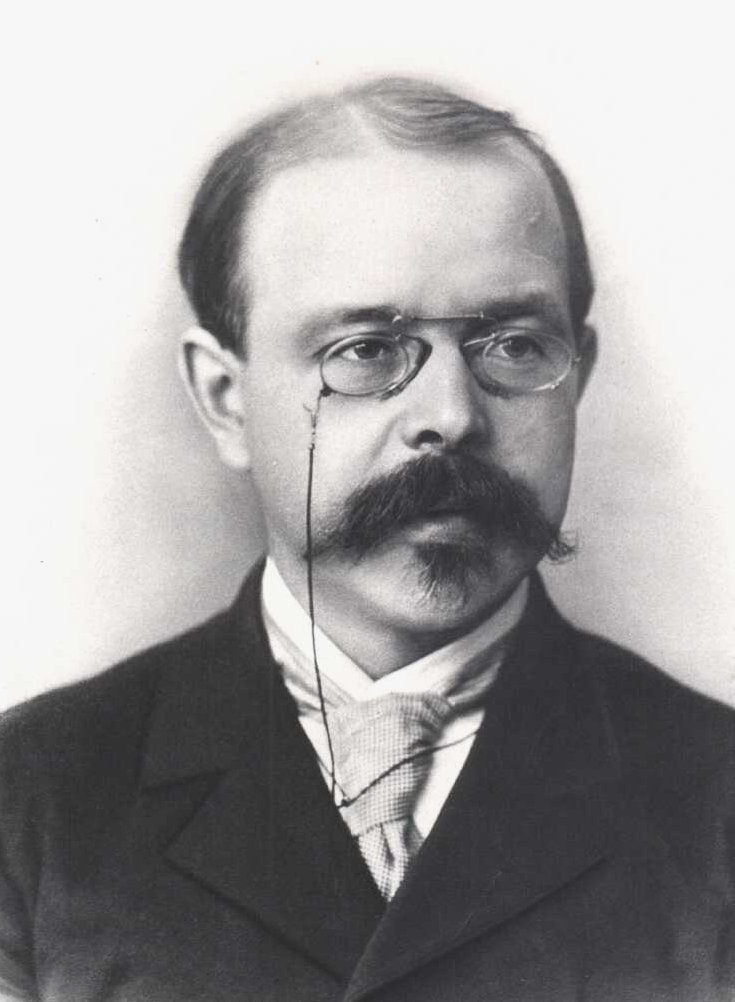
\includegraphics[width=\linewidth]{images/book2/nernst.jpg}
\end{minipage}\hfill
\begin{minipage}[t]{0.74\linewidth}\vspace{0pt}
Walther Nernst (1864--1941), aquí a los veinticinco años, en 1889. La
ecuación de esta sección, que relaciona la tensión de una pila con las
concentraciones de sus iones, lleva su nombre, y también un tercer
principio de la termodinámica que se encuentra en el volumen del segundo
año. (Fotografía: Smithsonian Libraries, dominio público, Wikimedia
Commons.)
\end{minipage}
\end{history}

\section{Predecir las reacciones redox}

\begin{method}[Predecir una reacción redox]\label{met:b1:nernst:predict-redox}
\begin{enumerate}
  \item Se sitúan los pares en una escala vertical de \omterm{def:b1:nernst:electrode-potential}{potenciales
        estándar}, con los \omterm{def:b1:nernst:couple}{oxidantes} a la izquierda y los \omterm{def:b1:nernst:couple}{reductores} a la
        derecha.
  \item El \omterm{def:b1:nernst:couple}{oxidante} más fuerte presente ($E^\circ$ más alto) reacciona
        con el \omterm{def:b1:nernst:couple}{reductor} más fuerte presente ($E^\circ$ más bajo): la
        flecha que baja del \omterm{def:b1:nernst:couple}{oxidante} al \omterm{def:b1:nernst:couple}{reductor} y vuelve a subir hacia
        los productos dibuja una gamma griega, $\gamma$.
  \item La reacción está favorecida ($K > 1$) cuando el par del \omterm{def:b1:nernst:couple}{oxidante}
        está por encima del del \omterm{def:b1:nernst:couple}{reductor}; en la práctica es \omterm{def:b1:extent-q-and-k:quantitative}{cuantitativa}
        cuando la diferencia supera unos \qty{0.25}{V} para un electrón
        intercambiado.
\end{enumerate}
\end{method}

\begin{omfigure}
\begin{tikzpicture}[font=\small, >={Stealth}, y=2.6cm]
  \draw[->, thick] (0,-1.0) -- (0,1.85) node[above] {$E^\circ$ (V)};
  \foreach \e/\o/\r in {-0.76/\ce{Zn^2+}/\ce{Zn}, 0/\ce{H+}/\ce{H2},
      0.34/\ce{Cu^2+}/\ce{Cu}, 0.77/\ce{Fe^3+}/\ce{Fe^2+},
      1.36/\ce{Cl2}/\ce{Cl-}, 1.51/\ce{MnO4-}/\ce{Mn^2+}} {
    \draw (-0.12,\e) -- (0.12,\e);
    \node[anchor=east] at (-0.25,\e) {\o};
    \node[anchor=west] at (0.25,\e) {\r};
    \node[anchor=west, black!55, font=\scriptsize] at (2.0,\e) {\e};
  }
  \node[omProp] at (-1.0,1.85) {oxidantes};
  \node[omDef] at (1.1,1.85) {reductores};
  % the gamma: Cu2+ meets Zn below it on the other side
  \draw[omThm, very thick, ->, rounded corners=4pt] (-1.0,0.28) -- (-1.0,-0.42) -- (0.6,-0.70);
  \draw[omThm, thick, ->] (-0.5,0.40) to[bend left=40] (0.5,0.40);
  \draw[omThm, thick, ->] (0.5,-0.85) to[bend left=40] (-0.5,-0.85);
\end{tikzpicture}

{\small Una escala de \omterm{def:b1:nernst:electrode-potential}{potenciales estándar}. La regla de la gamma: el
\omterm{def:b1:nernst:couple}{oxidante} \ce{Cu^2+} reacciona con el \omterm{def:b1:nernst:couple}{reductor} \ce{Zn}, situado debajo de
él en el otro lado (flecha gruesa); \ce{Cu^2+} se reduce a \ce{Cu} (flecha
curva superior) y \ce{Zn} se oxida a \ce{Zn^2+} (flecha curva inferior).
La reacción inversa, \ce{Cu} con \ce{Zn^2+}, no está favorecida.}
\end{omfigure}

\begin{proposition}[Constante de equilibrio a partir de los potenciales estándar]\label{prop:b1:nernst:equilibrium-constant}
Para la reacción $\mathrm{Ox_1} + \mathrm{Red_2} \rightleftharpoons
\mathrm{Red_1} + \mathrm{Ox_2}$, que intercambia $n$ electrones,
\[
  \log K = \frac{n\,(E^\circ_1 - E^\circ_2)}{0.059}\quad\text{a \qty{25}{\celsius}} .
\]
\end{proposition}

\begin{proof}
En el equilibrio no circula corriente por una pila construida con los dos
pares: los dos electrodos tienen el mismo potencial, $E_1 = E_2$. Se
escribe la \omterm{thm:b1:nernst:nernst}{ecuación de Nernst} de cada uno con el mismo $n$: $E^\circ_1 + \frac{0.059}{n}\log
\frac{a(\mathrm{Ox_1})}{a(\mathrm{Red_1})} = E^\circ_2 + \frac{0.059}{n}\log
\frac{a(\mathrm{Ox_2})}{a(\mathrm{Red_2})}$, de modo que $\frac{n(E^\circ_1 -
E^\circ_2)}{0.059} = \log\frac{a(\mathrm{Red_1})a(\mathrm{Ox_2})}{a(\mathrm{Ox_1})
a(\mathrm{Red_2})} = \log K$, siendo las \omterm{def:b1:extent-q-and-k:activity}{actividades} las del equilibrio.
\end{proof}

Para la reacción de la pila Daniell, $\log K = 2(0.34 + 0.76)/0.059 = 37$:
el cinc reduce por completo los iones cobre. Para
\ce{2Fe^3+ + 2I- <=> 2Fe^2+ + I2},
$\log K = 2(0.77 - 0.53)/0.059 = 8.1$. De aquí se deduce el criterio del
método: con $n = 1$, una diferencia de \qty{0.25}{V} da $K = 10^{4.2}$.

\begin{proposition}[Combinación de potenciales]\label{prop:b1:nernst:combined-potentials}
Si los pares $\mathrm{A}/\mathrm{B}$ ($n_1$ electrones) y
$\mathrm{B}/\mathrm{C}$ ($n_2$) se combinan en $\mathrm{A}/\mathrm{C}$
($n_3 = n_1 + n_2$), entonces $n_3 E^\circ_3 = n_1 E^\circ_1 + n_2 E^\circ_2$.
Los potenciales no se suman; los potenciales ponderados por los
electrones, sí.
\end{proposition}

\begin{proof}
En una disolución que contiene A, B y C en equilibrio con un electrodo,
los tres pares tienen el mismo potencial $E$. Se multiplica la \omterm{thm:b1:nernst:nernst}{ecuación
de Nernst} del primero por $n_1$ y la del segundo por $n_2$ y se suman: la
\omterm{def:b1:extent-q-and-k:activity}{actividad} de B se cancela y $(n_1 + n_2)E = n_1E^\circ_1 + n_2E^\circ_2 +
0.059\log\frac{a(\mathrm{A})}{a(\mathrm{C})}$, que es $n_3$ veces la
\omterm{thm:b1:nernst:nernst}{ecuación de Nernst} de A/C con el $E^\circ_3$ enunciado.
\end{proof}

Cobre: $2E^\circ(\ce{Cu^2+}/\ce{Cu}) = 0.16 + 0.52 = 0.68$, de modo que
$E^\circ(\ce{Cu^2+}/\ce{Cu}) = 0.34$~V, como en la tabla. Como
$E^\circ(\ce{Cu+}/\ce{Cu}) > E^\circ(\ce{Cu^2+}/\ce{Cu+})$, el ion
cobre(I) se oxida y se reduce a sí mismo, \ce{2Cu+ -> Cu^2+ + Cu}: no
sobrevive en el agua (\cref{ch:b1:e-ph-diagrams}).

\begin{proposition}[Electrodo de segunda especie]\label{prop:b1:nernst:second-kind}
Un hilo de plata recubierto de cloruro de plata en una disolución de
cloruro tiene el potencial
\[
  E = E^\circ(\ce{AgCl}/\ce{Ag}) - 0.059\log[\ce{Cl-}], \qquad
  E^\circ(\ce{AgCl}/\ce{Ag}) = E^\circ(\ce{Ag+}/\ce{Ag}) - 0.059\,\mathrm{p}K_s(\ce{AgCl}) .
\]
\end{proposition}

\begin{proof}
El hilo está en equilibrio con el \ce{Ag+} disuelto:
$E = E^\circ(\ce{Ag+}/\ce{Ag}) + 0.059\log[\ce{Ag+}]$, y el cloruro de
plata fija $[\ce{Ag+}] = K_s/[\ce{Cl-}]$. Al sustituir,
$E = E^\circ(\ce{Ag+}/\ce{Ag}) + 0.059\log K_s - 0.059\log[\ce{Cl-}]$.
\end{proof}

Numéricamente, $0.80 - 0.059 \times 9.75 = 0.22$~V, el valor de la tabla,
obtenido de forma independiente a partir de las entalpías libres. Un
electrodo así mide el cloruro o, a cloruro fijo, sirve de referencia.

\section{Ejercicios}

\begin{exercise}[$\star$]\label{exo:b1:nernst:1}
Dese el \omterm{def:b1:nernst:oxidation-number}{número de oxidación} del átomo subrayado: \ce{\underline{N}H3},
\ce{\underline{N}O3-}, \ce{\underline{S}O4^2-}, \ce{H2\underline{O}2},
\ce{\underline{Cr}2O7^2-}, \ce{\underline{Cl}O-}, \ce{\underline{Fe}3O4}
(media), \ce{\underline{C}H3OH}.
\end{exercise}

\begin{exercise}[$\star$]\label{exo:b1:nernst:2}
Ajústense en medio ácido las \omterm{def:b1:nernst:couple}{semiecuaciones} de \ce{Cr2O7^2-}/\ce{Cr^3+},
\ce{H2O2}/\ce{H2O}, \ce{O2}/\ce{H2O2} y \ce{SO4^2-}/\ce{SO2}.
\end{exercise}

\begin{exercise}[$\star$]\label{exo:b1:nernst:3}
Escríbase la \omterm{thm:b1:nernst:nernst}{ecuación de Nernst} de \ce{Zn^2+}/\ce{Zn}, \ce{Cl2}/\ce{Cl-},
\ce{O2}/\ce{H2O} y \ce{Hg2Cl2}/\ce{Hg}. Calcúlese el potencial de una
lámina de cinc en sulfato de cinc de \qty{0.010}{mol/L}.
\end{exercise}

\begin{exercise}[$\star$]\label{exo:b1:nernst:4}
Una pila Daniell contiene \ce{Zn^2+} a \qty{0.10}{mol/L} y \ce{Cu^2+} a
\qty{0.010}{mol/L}. Calcúlense el potencial de cada electrodo y la \omterm{def:b1:nernst:cell}{tensión
de la pila}, y dígase qué electrodo es el \omterm{def:b1:nernst:cell}{ánodo}.
\end{exercise}

\begin{exercise}[$\star\star$]\label{exo:b1:nernst:5}
Ajústese \ce{MnO4- + Fe^2+} en medio ácido, calcúlese su constante de
equilibrio y dígase si puede servir para una valoración.
\end{exercise}

\begin{exercise}[$\star\star$]\label{exo:b1:nernst:6}
¿Cuáles de estos metales se disuelven, desprendiendo hidrógeno, en un
ácido de \qty{1}{mol/L} que no es él mismo \omterm{def:b1:nernst:couple}{oxidante} (el ácido
clorhídrico): Mg, Zn, Fe, Ni, Pb, Cu, Ag? Escríbanse las reacciones y
calcúlese $\log K$ para el magnesio y para el hierro.
\end{exercise}

\begin{exercise}[$\star\star$]\label{exo:b1:nernst:7}
Las yodometrías usan \ce{I2 + 2S2O3^2- -> 2I- + S4O6^2-}. Calcúlese su
constante a partir de la tabla. ¿Es \omterm{def:b1:extent-q-and-k:quantitative}{cuantitativa}?
\end{exercise}

\begin{exercise}[$\star\star$]\label{exo:b1:nernst:8}
A partir de $E^\circ(\ce{Fe^2+}/\ce{Fe}) = -0.41$~V y $E^\circ(\ce{Fe^3+}/\ce{Fe^2+})
= 0.77$~V, calcúlese $E^\circ(\ce{Fe^3+}/\ce{Fe})$. Demuéstrese que los
iones hierro(III) reaccionan con el hierro metálico y calcúlese la
constante.
\end{exercise}

\begin{exercise}[$\star\star$]\label{exo:b1:nernst:9}
Demuéstrese que el potencial del par \ce{O2}/\ce{H2O} a \qty{1}{bar} de
oxígeno es $1.23 - 0.059\,\mathrm{pH}$, y el del par \ce{H+}/\ce{H2} a
\qty{1}{bar} de hidrógeno, $-0.059\,\mathrm{pH}$. ¿Cuál es la tensión de
una pila de combustible de hidrógeno--oxígeno? ¿Depende del pH?
\end{exercise}

\begin{exercise}[$\star\star\star$]\label{exo:b1:nernst:10}
El ion cobre(I). Con la tabla, demuéstrese que \ce{Cu+} se dismuta en el
agua, y calcúlense la constante de \ce{2Cu+ <=> Cu^2+ + Cu} y la
concentración de \ce{Cu+} que queda en equilibrio con cobre metálico y
\ce{Cu^2+} a \qty{0.10}{mol/L}.
\end{exercise}

\begin{exercise}[$\star\star\star$]\label{exo:b1:nernst:11}
Una pila \ce{Ag} $|$ \ce{Ag+} (\qty{1.0e-3}{mol/L}) $\|$ \ce{Ag+}
(\qty{0.10}{mol/L}) $|$ \ce{Ag} tiene el mismo par en los dos lados.
Calcúlese su tensión, identifíquense sus polos y descríbase cómo
evolucionan las concentraciones mientras suministra corriente. ¿Cuándo
se detiene?
\end{exercise}

\begin{exercise}[$\star\star\star$]\label{exo:b1:nernst:12}
El peróxido de hidrógeno. Calcúlese, a partir de la tabla, la constante
de \ce{2H2O2 -> 2H2O + O2} y explíquese por qué un frasco de agua
oxigenada es, sin embargo, estable durante meses. ¿Qué par de la tabla lo
hace \omterm{def:b1:nernst:couple}{oxidante} y cuál \omterm{def:b1:nernst:couple}{reductor}?
\end{exercise}

\section{Problema: el electrodo que mide el cloruro}

\begin{problem}[{Problema de fin de semana --- los números de oxidación
del par del cloruro de plata, una pila frente al electrodo de hidrógeno,
la medida del cloruro de una muestra de agua y el potencial estándar del
electrodo de plata--cloruro de plata}]
\label{pb:b1:nernst:1}
Un laboratorio de aguas mide el cloruro con un hilo de plata recubierto de
cloruro de plata, sumergido en la muestra y conectado a un \omterm{def:b1:nernst:reference-electrode}{electrodo de
referencia}. Datos a \qty{25}{\celsius}: $E^\circ(\ce{Ag+}/\ce{Ag}) = 0.80$~V,
$E^\circ(\ce{AgCl}/\ce{Ag}) = 0.22$~V, $E^\circ(\ce{Hg2Cl2}/\ce{Hg}) =
0.27$~V, $\mathrm{p}K_s(\ce{AgCl}) = 9.75$, $RT\ln 10/F = 0.059$~V,
$M(\ce{Cl}) = \qty{35.5}{g/mol}$.

\medskip
\noindent\textbf{Parte I --- El par.}
\begin{enumerate}
  \item Dese el \omterm{def:b1:nernst:oxidation-number}{número de oxidación} de la plata en Ag, \ce{Ag+} y
        \ce{AgCl}, y el del cloro en \ce{AgCl} y \ce{Cl-}.
  \item Escríbase la \omterm{def:b1:nernst:couple}{semiecuación} del par \ce{AgCl}/\ce{Ag}.
  \item Escríbase su \omterm{thm:b1:nernst:nernst}{ecuación de Nernst}.
  \item Explíquese por qué el potencial solo depende de la concentración
        de cloruro.
  \item ¿Cuál es el potencial del electrodo en cloruro de
        \qty{1.0}{mol/L}?
  \item Calcúlese en cloruro de \qty{0.010}{mol/L}.
\end{enumerate}

\medskip
\noindent\textbf{Parte II --- Una pila frente al electrodo de hidrógeno.}
\begin{enumerate}[resume]
  \item Escríbase la pila formada por el \omterm{def:b1:nernst:electrode-potential}{electrodo estándar de hidrógeno} y
        el electrodo de cloruro de plata en cloruro de \qty{0.10}{mol/L}.
  \item ¿Qué electrodo es el polo positivo?
  \item Calcúlese la \omterm{def:b1:nernst:cell}{tensión de la pila}.
  \item Escríbase la reacción que tiene lugar cuando la pila suministra
        corriente.
  \item Calcúlese su constante de equilibrio.
  \item ¿En qué sentido se desplazan los electrones por el hilo?
\end{enumerate}

\medskip
\noindent\textbf{Parte III --- Medir el cloruro.}
La referencia es un electrodo de calomelanos en cloruro de potasio de
\qty{1.0}{mol/L}.
\begin{enumerate}[resume]
  \item ¿Cuál es el potencial de la referencia?
  \item Para una muestra de \qty{1.0e-3}{mol/L} de cloruro, ¿qué electrodo
        es el polo positivo y cuál es la tensión?
  \item Exprésese la tensión $U$ (electrodo de plata menos referencia) en
        función de $[\ce{Cl-}]$.
  \item Una muestra da $U = \qty{0.115}{V}$. Calcúlese su concentración de
        cloruro en \unit{mol/L} y en \unit{mg/L}.
  \item Un error de \qty{1}{mV} en $U$, ¿qué error relativo da en la
        concentración?
  \item ¿Por debajo de qué concentración de cloruro deja el electrodo de
        seguir la \omterm{thm:b1:nernst:nernst}{ecuación de Nernst}, al disolverse su cloruro de plata?
\end{enumerate}

\medskip
\noindent\textbf{Parte IV --- ¿De dónde sale 0.22 V?}
\begin{enumerate}[resume]
  \item Escríbase la \omterm{thm:b1:nernst:nernst}{ecuación de Nernst} de \ce{Ag+}/\ce{Ag}.
  \item En presencia de cloruro de plata sólido, exprésese $[\ce{Ag+}]$ en
        función de $[\ce{Cl-}]$.
  \item Dedúzcase el potencial del hilo de plata en función de
        $[\ce{Cl-}]$.
  \item Identifíquese $E^\circ(\ce{AgCl}/\ce{Ag})$ en esa expresión.
  \item Calcúlese a partir de $E^\circ(\ce{Ag+}/\ce{Ag})$ y del
        $\mathrm{p}K_s$, y compárese con el valor de la tabla.
  \item Dese el \omterm{def:b1:nernst:electrode-potential}{potencial estándar} del electrodo de plata--cloruro de plata
        con dos decimales.
\end{enumerate}
\end{problem}
